\documentclass{article}

\usepackage{amsmath}
\usepackage[margin=3cm]{geometry}
\usepackage{graphicx}
\usepackage{hyperref}
\usepackage{listings}
\usepackage{minted}
\usepackage[nodayofweek]{datetime}

\title{
    \textbf{Programming Club}\\
    Sudoku \\
}
\author{Volker Seeker}
\date{\today}

\begin{document}
    \maketitle

\setlength{\parskip}{1em}
\setlength{\parindent}{0em}

    \section{Introduction}
    In this problem you are asked to create a Sudoku game and algorithms
    to solve, rank and generate game fields automatically.

    As always, we have provided you with some guidance on how to get started
    with the problem, but you are welcome to deviate and follow your own interests.

    \subsection{Rules}
    A Sudoku game is played on a grid of 9x9 fields which can be subdivided in 9 3x3
    sub-fields. Each field can contain a number between 1 and 9. For a given Sudoku
    game, some of the fields are already pre-populated with numbers.

    The goal of the game is to find a number for every field of the grid while following
    a given set of rules:

    \begin{itemize}
        \item Every number only appears once per row.
        \item Every number only appears once per column.
        \item Every number only appears once in every 3x3 sub-grid.
    \end{itemize}

    Here is an example of a Sudoku game at the start and once it is completely solved:

    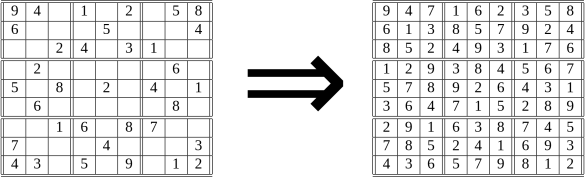
\includegraphics[width=1\textwidth]{game_example}


    \section{Part 1: The Game}

    \begin{enumerate}
        \item Create a data structure to hold a Sudoku grid with 9x9 fields. Each of the
            fields should be able to contain a number between 1 and 9 or it can be empty.
        \item Write a method to test for a single field of the grid whether its current 
            number is set according to the rules specified above.
        \item Write a method to load a Sudoku game from a file. Each line of the file
            corresponds to a line of the Sudoku grid. Numbers for each field can be
            separated by a white space. Empty fields can be represented by a 0.
        \item Write an interactive program to play the game. This can be a simple command
            line interface or a fancy GUI.
    \end{enumerate}

    \section{Part 2: Automatic Solving}

    \begin{enumerate}
        \item Write a method which solves the Sudoku using a backtracking algorithm. You
            can find a description of the algorithm and an example here: 
            
            \url{https://www.geeksforgeeks.org/backtracking-set-1-the-knights-tour-problem/}

            Keep in mind that some fields of a Sudoku game might already by pre-populated
            and should not be changed.

        \item Can you think of another way to solve the Sudoku other than backtracking?
    \end{enumerate}

    \section{Part 3: Ranking a Game}

    \begin{enumerate}
        \item Extend the backtracking algorithm so that it finds not just one but every
            possible solution for a given Sudoku game.
        \item Write an algorithm which calculates a rank for a Sudoku game based on the
            following rules and returns it:
            \begin{itemize}
                \item The fewer solutions a Sudoku game has the higher its rank, i.e.\ a game
                    with $n + 1$ solutions has a lower rank than a game with $n$ solutions.
                    Since a solvable Sudoku game must have at least one solution, $n=1$ is the
                    optimum.
                \item Should two Sudoku games have the same number of solutions, the one with 
                    less given numbers should be ranked higher than the one with more
                    given numbers. In the (unrealistic) best scenario, all 81 fields can be free.
            \end{itemize}
        \item Write a program which reads multiple Sudoku games, assigns a rank to each of them
            and returns the one with the highest rank.
    \end{enumerate}
    
    \section{Part 4: Game Generation}

    Using the ranking method implemented in the previous part as cost function, write a 
    Sudoku game generator using \textit{simulated annealing}. You can find a good explanation
    of this algorithm here:

    \url{http://katrinaeg.com/simulated-annealing.html}

    You can follow these guidelines to get started:
    \begin{itemize}
        \item The generator starts at a fully and correctly solved Sudoku field
        \item Every step of the algorithm going towards the solution can either remove
            a number or add one.
        \item Use the rank of your intermediate solution to check whether you reached the
            optimum yet or at least a sufficiently good rank.
        \item Intermediate solutions are only accepted if they are following Sudoku rules.
    \end{itemize}

    \section{Sample Sudokus}
    You can find some sample game files including unsolvable Sudokus on the github page:

    \url{}

\end{document}
